% ======================================================================
% Einrückungen und Zeilenabstand
% ======================================================================
\setlength\parindent{0pt}
\setlength\parskip{2 pt plus 1 pt minus 1 pt}
% ======================================================================


% ======================================================================
% Seitenlayout
% ======================================================================
\geometry{ %
  head     = 1.2 cm, %
  headsep  = 1.4 cm, %
  top      = 4.5 cm, %
  right    = 2.4 cm, %
  left     = 2.4 cm, %
  foot     = 1.0 cm, %
  footskip = 2.0 cm, %
  bottom   = 3.0 cm
}
% ======================================================================


% ======================================================================
% Helvetica für alles
% ======================================================================
\renewcommand{\familydefault}{\sfdefault}
% ======================================================================


% ======================================================================
% Kopf- und Fußzeilen
% ======================================================================
\pagestyle{fancy}

% Keine Linien
\renewcommand{\headrulewidth}{0pt}
\renewcommand{\footrulewidth}{0pt}

% Oben links: Dreizeiler, 1 cm hoch
\fancyhead[L]{\hspace{-1 mm}\resizebox{!}{1 cm}{%
  \begin{tikzpicture}
  \node[inner sep = 0 pt, outer sep = 0, text width = 10 cm, align = left] at (0, 0) %
  {%
      \fontfamily{phv}\selectfont\color{tum blue}%
      Lehrstuhl für Regelungstechnik\\
      TUM School of Engineering and Design \\
      Technische Universität München
  };
  \end{tikzpicture}
}}
% Oben mitte: Leer
\fancyhead[C]{}
% Oben rechts: TUM-Logo, 1 cm hoch
\fancyhead[R]{\resizebox{!}{1 cm}{%
  \begin{tikzpicture}
    \path[fill=tum blue]
      (0.1649, 0.8021) -- (0.0000, 0.8021) --
      (0.0000, 1.0000) -- (0.7347, 1.0000) --
      (0.7347, 0.2028) -- (0.9109, 0.2028) --
      (0.9109, 1.0000) -- (1.8716, 1.0000) --
      (1.8716, 0.0000) -- (1.6653, 0.0000) --
      (1.6653, 0.7930) -- (1.4884, 0.7930) --
      (1.4884, 0.0000) -- (1.2842, 0.0000) --
      (1.2842, 0.7930) -- (1.1098, 0.7930) --
      (1.1098, 0.0000) -- (0.5326, 0.0000) --
      (0.5326, 0.8021) -- (0.3642, 0.8021) --
      (0.3642, 0.0000) -- (0.1663, 0.0000) --
      cycle;
  \end{tikzpicture}
}\hspace{-1 mm}}

% Unten links: Info
\fancyfoot[L]{%
  \begin{tikzpicture}
    \small
    \node[inner sep = 0 pt, outer sep = 0, align = left] at (0, 0) %
      {
        {\BetreuerWort}:~{\BetreuerName}\\%
        {\BetreuerBuero}, \, \Telefon \, +49\,89\,289\,{\BetreuerDurchwahl}\\%
        {\href{mailto:\BetreuerEMail}{\texttt{\BetreuerEMail}}}%
      };
  \end{tikzpicture}
}
% Unten mitte: Leer
\fancyfoot[C]{}
% Unten rechts: Seitennummer
\fancyfoot[R]{%
  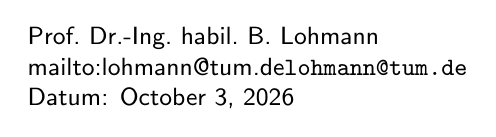
\begin{tikzpicture}
    \small
    \node[inner sep = 0 pt, outer sep = 0, align = left] at (0, 0) %
      {%
        Prof.~Dr.-Ing.~habil.~B.~Lohmann\\%
        {\href{mailto:lohmann@tum.de}{\texttt{lohmann@tum.de}}}\\%
        Datum: \today
      };
  \end{tikzpicture}
}
% ======================================================================


% ======================================================================
% SI Einheiten -- deutscher Stil
% ======================================================================
\sisetup{
    detect-all            = true,
    per-mode              = symbol,
    binary-units          = true,
    retain-zero-exponent  = true,
    exponent-product      = \cdot,
    locale                = DE
}
% ======================================================================


% ======================================================================
% hyperref
% ======================================================================
\hypersetup{
    pdffitwindow    = false,
    pdfstartview    = FitH,
    pdftitle        = {{\TypDerArbeit}: {\TitelDerArbeit}},
    pdfauthor       = {Lehrstuhl für Regelungstechnik},
    pdfkeywords     = {{\TypDerArbeit}, %
                       {\TitelDerArbeit}, %
                       Technische Universität München, %
                       Technical University of Munich, %
                       TUM, %
                       Chair of Automatic Control, %
                       Lehrstuhl für Regelungstechnik %
                      },
    pdfnewwindow    = false,
    colorlinks      = false,
    linkcolor       = black,
    urlcolor        = black,
    citecolor       = black,
    allbordercolors = black!10,
    urlcolor        = black,
}
% ======================================================================


% ======================================================================
% cleveref
% ======================================================================
\crefformat{equation}{{#2(#1)#3}}
\Crefformat{equation}{{#2(#1)#3}}
% ======================================================================


% ======================================================================
% pgfplots
% ======================================================================
\pgfplotsset{compat = newest} % use the newest version
% ======================================================================
